\documentclass[sigconf]{acmart}
\usepackage{amsmath}
\usepackage{amssymb}
\usepackage{amsfonts}
%\usepackage{graphics}
%\usepackage{curves}
%\usepackage{tikz}
%\usetikzlibrary{backgrounds}
%\usetikzlibrary{snakes} \documentclass{report}
%\usepackage{amsmath}
%\usepackage{amssymb}
%\usepackage{amsfonts}
%\usepackage{graphics}
%\usepackage{curves}
%\usepackage{tikz}
%\usetikzlibrary{backgrounds}
%\usetikzlibrary{snakes}
%\usepackage{setspace}
%\doublespacing
%\usepackage{lscape}
%\usepackage{booktabs}
%\usepackage{longtable}
\usepackage{hyperref}
\usepackage{url}
\usepackage{color}

\author{ABMSPECSIG Group}
\title{Wealth dynamics in the presence of network structure and primitive cooperation}
\bibliographystyle{plain} 
\begin{document}

\maketitle
\begin{abstract}
We study wealth accumulation dynamics in a population of heterogeneously mixed agents with a capacity for a certain primitive form of cooperation enabled by static network structures. Despite their simplicity, the stochastic dynamics generate inequalities in wealth reminiscent of real world social systems even in a fully mixed population. A simple form of cooperation is introduced and is shown to enhance the viability of agents By embedding such dynamics in a network, the impact of social structures on the origins and persistence of inequality can be teased out easily. The models developed here complement traditional modeling approaches based on grid worlds.   

\end{abstract}
\section{Introduction}
In recent years, concerns and debates surrounding wealth inequality and socioeconomic mobility have been one of the few unifying issues dominating the extremely polarized public spheres of the Global North. While economic and political inequality used to be discussed in not so mainstream heterodox economics circles, the contentious discussions on the topic within mainstream economics since the publication of Piketty's book~\cite{piketty2017capital} suggests a lack of consensus about very basic foundational questions like the origins and persistence of economic inequality. Not surprisingly, traditional theories and tools of macro and micro economics are now being diagnosed for their limitations. Simultaneously, insights from related disciplines, along with novel scientific inquiry models not usually associated with traditional econometrics, are being taken more seriously. The work presented here shares this spirit by integrating substantive ideas from anthropology, economic sociology~\cite{granovetter2017society} and urban sociology~\cite{sampson2012great} and using modeling approaches from computational social science~\cite{hedstrom2018}, computational economics~\cite{tesfatsion} and analytical sociology~\cite{hedstrom2011oxford} to understand the origins of inequality in a simple model of wealth dynamics in the presence of social structures.    
% SD: citation for "anthropology," the first element of the last sentence's list? Grief and/or White?

The current work originated in our attempts to incorporate and tease out the effects of social structures in simple models of wealth dynamics in the presence of environmental stochasticity, and a simple form of resource pooling. Specifically, we are interested in studying how structure and dynamics interact to produce and sustain inequality, and influence robustness to scarcity shocks. We answer the former question using Gini coefficients; the latter question is answered using survival time type analysis. As we discuss in section 3, while Gini was found to be of limited value, survival time analysis produced more insights on both questions of inequality and robustness. 

These models were inspired by our search for analogs of the grid world agent-based models (ABMs) of Friesen and Mudigonda~\cite{srimil} where foraging agents that pool their resources were shown to on-average outperform non-pooling agents. The original model used foraging to mix the population and create opportunities for interaction, and, when certain conditions were met, allowed resource sharing. Our model achieves agent interaction by postulating a static network structure which partially mixes the agents. Of primary interest is whether network effects alone can generate and sustain differences in economic outcomes of otherwise homogeneous agents.  

The original model drew its inspiration from historical sociology, in Katz's influential study of middle of 19th century Hamilton, Canada~\cite{katz2013people}. Retaining this original motivation, we draw additional inspiration from economic sociology, in the work of Granovetter~\cite{granovetter2005}; urban sociology, in the work of Sampson~\cite{sampson2002} and others; and in anthropology, in the work on cooperation in small to medium scale societies~\cite{avner1994,white2011kinship}. The geographic and economic scale of the systems, the nature of social actors and time period of interest are all very different from the ones used to develop models of representative agents in macroeconomics~\cite{benhabib2018}, making the similarity between macroeconomic wealth dynamics models and our models not comparable without further justification. Elaborating on the interplay of conceptual and methodological ideas among these disciplines is beyond the scope of this article. Instead, we anchor this work in economic sociology and revisit the insights from the above disciplines in the article's concluding section.

The important role played by social structures or non-economic structures in determining economic outcomes of individuals in a society is not in doubt~\cite{granovetter2005,jackson_rev2017}. Still, in the absence of a unifying foundation for sociology and economics, the full impact of this two-way interpenetration of economic and social structures is demonstrated only on a case-by-case basis. The language of social and economic networks affords a first principle integration by simplifying the non-trivial concept of social and economic structure~\cite{martin_lee} to only dyadic relations. 

As mentioned earlier, macroeconomic models are ill-suited to the study of collective phenomena at an intermediate level. Hence, alternative explanations of aggregate phenomena that match the expressiveness of economic models are required. Analytical sociology~\cite{ch1as_hdbk}, with its emphasis on explanation of collective emergent phenomena using mathematically formulated social mechanisms~\cite{ch2as_hdbk,ch11as_hdbk} anchored at the individual level, is an ideal candidate for this purpose. It is particularly powerful when combined with computational simulation, because when mathematically-formulated models reach even a modest level of complexity, they often become analytically intractable. Simulation \textit{in silico} can yield approximate results for these more complex scenarios, which supplement the exact results reached by traditional methods.

Models constructed here, like those used in scientific inquiry in general, serve a specific purpose. In this work, we construct simple toy models to reproduce certain aspects of non-trivial wealth inequality distributions in the presence and absence of primitive forms of cooperation, clearly delineating the role of network structure in generating wealth inequality. We make no suggestions that these models \textit{explain} the phenomena of interest; we are only interested in constructing the simplest possible models, with no detailed empirical grounding, but with the potential to generate realistic looking inequality distributions. In doing so, we aspire to shed light on the \textit{true} social and economic mechanisms underlying the genesis and persistence of economic inequality, and network structure alone can produce large differences in economic outcomes. 


\label{giniKindaSucks}
% SD: In light of recent discussions, we may want to downplay Gini and up-play the robustness of agents to exogenous shocks.
The phenomenon under scrutiny is the emergence and evolution of economic inequality in societies with non-trivial social structures that enable economic interactions and cooperation mechanisms. The model we use to answer questions surrounding this phenomenon must possess a dynamic model of wealth accumulation, a model of social structure, and a suitably useful measure of inequality. The dynamics are modeled as Brownian noise driven linear dynamical systems, here constant growth rate; the structure is modeled by networks, here random graphs; the measures of inequality used are Gini coefficients, and survival time distributions of agents in response to lack of resources. Although both the dynamical system and the network model are quite well understood, the precise interplay of structure and dynamics produces interesting emergent wealth distributions and robustness to scarcity. To the best of our knowledge, this specific combination of network structure and social dynamics has not been discussed in the computational social science (CSS) or mathematical sociology literature, and we consider this the primary contribution of this work. 

Apart from enabling interactions between social actors, social structures like institutions also shape the form of cooperation and coordination mechanisms. The institutions can take the form of economic institutions, like banks and cooperatives; or the form of norms, like resource-sharing practices in societies. The original SriMil model~\cite{srimil}consists of a simple resource pooling arrangement where aggregates of agents pool their excess wealth in a common institution called ``proto-institutions,'' agreeing to provide this saved resource to individual agents in times of need. The model of resource pooling used in this work is identical to the SriMil model. 

The analysis to be presented in later sections focuses only on homogeneous agents with simple drift-diffusion dynamics on Erd\H{o}s-R\'{e}nyi network models (ER); space constraints unfortunately prevent us from repeating the analysis on other standard \textit{textbook} networks like scale-free and small-world networks. We discuss empirical evidence for the role of social network structures in the concluding section of this paper, motivating the need for more expressive social network models. 


In the next section, we discuss the mathematical formulation of the model. In section 3, we present the analysis of our simulation experiments, summarize key findings and discuss why we chose the \texttt{julia} programming language~\cite{Julia-2017} for our implementation. In section 4, we discuss the limitations of our simple models, extensions to dynamics and networks more expressive than the ones presented here, and planned future work. 

Before discussing our model in greater mathematical detail, we discuss the model qualitatively, contrasting them with more familiar modeling approaches. The model presented here has much in common with models used in social reality inspired models in statistical physics~\cite{redner2001guide}, dynamic process models in network science~\cite{newman2018networks}, and computational social science and agent-based models~\cite{abm_review}; however, our modeling philosophy is somewhere at the interface of agent-based computational economics (ACE)~\cite{tesfatsion} and analytical sociology (AS)~\cite{ch1as_hdbk,ch2as_hdbk}. In ACE, we acknowledge its aspiration to develop bottom-up models of economic systems at all scales but restrain from its enthusiastic use of complex but well-calibrated detailed models of markets and agents~\cite{tesfatsion2017}. In AS, we assent its focus on social mechanisms in explaining social phenomena, but instead rely on simplified mechanisms with few parameters~\cite{ch11as_hdbk} with the specific goal of extracting insights from \textit{stylized} models.       

More specifically, from statistical physics, we borrow the dynamics: diffusion models and associated first-passage time techniques; from network science, we borrow the structural aspects: Erd\H{o}s-R\'{e}nyi network (ER) models; and from non-equlibrium statistical physics, CSS and ACE, we borrow a form of cooperation: the concept of coalescence, institution and coordination. 


\section{Model}
The model of cooperative wealth accumulation constructed here is best thought of as a stochastic interacting particle system infused with economic sociological semantics. The particle evolves according to an one dimensional diffusion process with constant drift and is driven by a Brownian noise with boundary condition at the origin corresponding to particle absorption. After crossing a pre-determined threshold in state space, particles above the threshold follow a protocol and coalesce together. In an ensemble of otherwise identical particles, a given particle may coalesce with a subset of other particles. This mixing characteristic is encoded via a graph. Both the conjoined particles and individual particles die upon crossing the origin. This model of interacting diffusing particles can be provided with substantive semantics as follows. 

%Might be nice to put a nice table here 
The one dimensional state space of the particle is identified with the wealth of an social actor (agent). We consider a homogeneous population where all agents are required burn their wealth at a constant specified rate in order to survive. In addition, the agents all gain wealth at a constant rate. The resource draining rate and the resource gaining rate are additive and constitute the drift of the diffusion process. The environmental contingency is modeled by a Brownian noise of a specified intensity. Upon crossing a specific wealth threshold, agents can coalesce to form a cooperative unit deciding to pool their resources and their environmental contingencies into a single unit which we call a \textit{proto-institution} (proto). The mixing characteristic of this ensemble is the social network (here ER model).          

The questions of interest to us, emergence and persistence of inequality and robustness to scarcity, in the presence of social structure and uncertain environmental conditions, map onto questions about the stochastic dynamical system (SDS). Inequality can be quantified using Gini coefficients of the particle ensemble's state space. Robustness to scarcity can be measured using survival time analysis for the particles to reach the absorbing boundary at the origin, by turning off the appropriate drift terms in the dynamics. 

\subsection{Mathematical formulation}
The discussion of SDS closely follows ~\cite{redner2001guide}\footnote{The use of such analysis for studying wealth dynamics was presented by one of the authors at CSSA18 ~\cite{rv}. Unlike the finite interval dynamics used there, the dynamics here take place on a semi-infinite line.}

The SDS can be defined through a stochastic differential equation of the form 

\begin{equation}\label{ddm}
dx(t) = vdt + \sqrt{2D} dw
\end{equation}

\noindent where $v$ is the wealth growth rate (the difference of the income and metabolic rate of the agent) and $D$ is the intensity of the Brownian process (white noise process) $w$. $x(t)$ is the state of the particle (wealth) at time $t$. The dynamics can be started at a any initial point $x_0 > 0$. 

While equation (\ref{ddm}), in its discretized form, is the basis for simulations, other formulations are used~\cite{redner2001guide,rv}\footnote{These formulations make use measure theoretical probability to convert SDEs to partial differential equations known as Fokker-Planck equations.  The provide numerical and closed form estimates of probability density, survival time probabilities and other quantities of importance.}.

\noindent For a single particle, the probability of survival $S(t)$ and the expected probability of reaching the origin can be calculated and are functions of $x_0$, $v$ and $D$. For example, the expected probability of a particle reaching the origin ($\mathcal{E}(x_0)$), when starting at $x_0$ is given by 

\begin{equation}\label{e}
\mathcal{E}(x_0) = \begin{cases}
e^{-v x_0/D} \text{, } & \text{ for } v > 0 \\
1 \text{, } & \text{ for } v \leq 0 \\
\end{cases}
\end{equation}  

\noindent That is, there is always a non-zero probability of reaching the particle, even when there is a constant positive drift away from the origin; and, the return to origin is certain for negative or zero drift.  Similarly, survival probability, $\mathcal{S}(t)$ is given by 

\begin{equation}\label{s}
\mathcal{S}(t) = \begin{cases}
1 - e^{-v x_0/D}\text{, } & \text{ } v >0 \\
\sqrt{\frac{4D}{\pi v^2 t} e^{-v^2 t/4 D}}\text{, } & \text{ } v \leq 0 \\
\end{cases}
\end{equation}

Since the particles are independent, they are independent dynamical systems; proto formation is a higher level construct imposed on this system and is a constraint on what states are considered viable and what are not. Consider two particles $x_1$ and  $x_2$ that have crossed the threshold for coalescence $x_{thresh}$. After the coalescence event, the state (wealth) of individual particles $x_1(t)$ and  $x_2(t)$ is not important; only the aggregate wealth of the coalescent (proto) is important. As long as $x_1(t) + x_2(t) >0$, both particles survive. Effectively, the proto is a two-dimensional SDS. Since the wealth of the proto ($p_{12}$)is additive, the aggregate wealth $p_{12} = x_1(t) + x_2(t) $. The dynamical variable satisfies an SDE\footnote{The result follows from the additivity properties of white noise.}

\begin{equation}\label{pddm}
dx(t) = 2vdt + \sqrt{2*2D} dw
\end{equation}

As one can see, only the coefficient of drift and diffusion in equations (\ref{ddm}) and (\ref{pddm}) are different. So, the corresponding expressions for $\mathcal{E}(x_0)$ and $\mathcal{S}(t)$ are suitably scaled. This has implications for both Gini coefficient calculations and survival analysis calculations. 

For such ensemble of particles, the primary driver of difference in paths (life histories) and wealth is the Brownian noise intensity $D$; greater the $D$. greater the diversity (and hence Gini). However, Gini is a measure that is dependent on absolute magnitude. So,  if the drift ($v$) is large, then the variation generated by
$D$ gets washed out by $v$\footnote{Preliminary investigations suggest that for simple non-network ensembles, Gini either stays close to $0$ or $1$. We suspect that this is because of the constant wealth growth rate used in our models, Gini is a partially useful measure. This is unlike in macroeconomic models where exponential growth rate gives rise a appearance of non-trivial Gini coefficients}.  On the other hand, the mathematical form of expressions for $\mathcal{S}(t)$ suggest a clear and non-trivial dependence of the $D$ and clear separation between the population of particles that are isolates and the population of particles that are in a proto. 

As the equations (\ref{e}) and (\ref{s}) show, all agents, irrespective of their starting intial condition and luck have a non-zero probability of dying. The paper that inspired this work ~\cite{srimil} emphasized studied inequality dynamics in the context of extreme scarcity in their foraging world. One can mimic this scarcity by simply turning of the income, leaving the agents to all inevitably die. The differential rate of death of the isolates and the non-isolates then become an important quantity. 

In the simulation experiments that we discuss next discusses various stages and stopping conditions. All these stages and transition times between them make sense in terms of the underlying dynamics of the particle ensemble. In each of the stages, the effective dynamics are different from each other but the form of the equations remain the same. 

To break the homogeneity of this particle ensemble, we propose to let the particles interact with only  a random subset of other populations. In other words, we embed the particles on a network (graph); particles interact (form proto) with only their neighbors. In this work, we focus on the simplest \textit{textbook} example of network: Erd\H{o}s-R\'{e}nyi network model~\cite{newman2018networks}. ER models has only one parameter $\lambda$, a Poisson parameter that determines the density of connections in the network, and in this setting, determines the number of particles available for a particle to coalesce and form protos. Commonsense reasoning suggests that a larger $\lambda$ parameter may help increase the average lifetimes of individual agents through by enabling greater likelihood of contact with other particles. 

Just as equations (\ref{e}) and (\ref{s}) offers insight about the role of dynamics, the key feature of ER models is the the formation of giant component at $\lambda=1$, allowing a finite fraction of the population to be connected, have cliques of very high order, and other useful properties guarantee proto formation in large fraction of the population.  

As its network properties are well-understood, wealth dynamics on such network allows us to understand more thoroughly, the interaction between dynamics and structure, and its role in global behavior. Still, a full analysis of this model remains to be completed and is part of a forthcoming work involving other more expressive network models. As we note subsequently, even this simple setting offers interesting insights,


\subsection{Implementation}


The model is realized in a discrete-time Julia simulation program, in which each agent is represented as a mutable struct (a dedicated area of memory whose contents change over time) that maintains its state. An agent's state includes its current amount of wealth and which proto (if any) it is a member of. Additionally, using the LightGraphs package~\cite{LightGraphs-2017}, each agent is associated with a node of a randomly generated ER graph. Protos are also represented as mutable structs, each of which contains a list of member agent IDs and a current wealth balance.

The simulation proceeds as follows. For configurable parameters
$N > 0$,
$\texttt{init\_max} > 0$,
$\texttt{salary} > 0$,
$m > 0$ (metabolic rate),
$t_p > 0$ (the ``proto threshold''),
$\sigma^2 \ge 0$ and
$0 \le \lambda \le 1$:

\begin{enumerate}
\itemsep.1em
\item Create $N$ agents, each with a random initial wealth (uniformly distributed from 0 to \texttt{init\_max}), and related to one another as per a random ER network with parameter $\lambda$.
\item \textbf{Stages 1 and 2\footnote{We define ``Stage 1'' as the period \textit{before} the first proto is formed, ``Stage 2'' as the period \textit{during} which protos are being formed}:} Repeat until all non-isolate agents\footnote{An \textbf{isolate} agent is one with no graph neighbors.} are members of a proto:
    \begin{enumerate}
    \itemsep.1em
    \item Each agent $A$ whose current wealth $\ge t_p$, and who is not currently a member of a proto, chooses at random one of its graph neighbors (call it $B$) whose wealth \textit{also} exceeds $t_p$. (If there are no such neighbors, proceed to the next agent.) If $B$ is already in a proto, have $A$ join $B$'s proto. If not, have $A$ and $B$ form a new proto.
    \item Each agent gains an amount of wealth equal to $(\texttt{salary} - m + \epsilon)$, where $\epsilon \sim \mathcal{N}(0,\sigma^2)$ (white noise).\footnote{Note that this ``gain'' could be negative, in which case the agent, and possibly its proto, may be subject to death exactly as in step (3).}
    \item Each agent \textit{that is in a proto} donates all its wealth in excess of $t_p$ to that proto's balance. (Agents not in a proto maintain their current wealth.)
    \end{enumerate}
    \item \textbf{Stage 3 (starvation):} Repeat until all agents are dead:
        \begin{enumerate}
        \itemsep.1em
        \item Each agent \textit{loses} an amount of wealth equal to $(m + \epsilon), \epsilon \sim \mathcal{N}(0,\sigma^2)$.
        \item If an agent's wealth would drop below zero as a result of this loss, and if it is not a member of a proto, it dies and is removed from the simulation. If it \textit{is} a member of a proto, it withdraws the necessary amount from its proto's balance to remain at zero wealth. If the proto does not have sufficient funds to cover the loss, both the agent and the proto die and are removed from the simulation.
        \end{enumerate}
\end{enumerate}

Various statistical counters are updated as the program executes so that its behavior can be analyzed post mortem. The main simulation loop can also be invoked from a ``parameter sweep'' program which executes it multiple times over a range of parameter values, in order to determine how the model's behavior changes in response to key parameters.

% cite Bootstrap?
We chose Julia for its flexible type system, its speed of execution, its ease of programming, and the availability of useful packages, such as LightGraphs, Gadfly~\cite{Gadfly-2018} (plotting), and Bootstrap (confidence intervals).  Additionally, Julia easily allows the programmer to invoke code from R packages when necessary, as we did for Gini coefficient calculation with the R package DescTools~\cite{DescTools-2019}.


\section{Verification}

We first verify that the simulation's output matches obviously expected
results. Then, in the following section, we investigate aspects of its behavior
which are not computable analytically in order to discover important
consequences of the model.


\subsection{Agent and proto life history}

For a sensible range of parameter settings, the life history of a single
simulation run follows an expected pattern. Assuming a positive growth rate
(\textit{i.e.}, salary > metabolic rate), each agent's wealth rises unsteadily
during stage 1, until eventually the first pair of neighboring agents who each
reach the threshold form a proto-institution. Throughout stage 2, these agents
contribute all wealth in excess of the threshold to that proto, and so their
proto's balance rises unsteadily while their personal wealth remains at the
constant threshold. Meanwhile, the other agents also reach the threshold at
various points in time, and also form or join protos, until every non-isolate
(that is, every node with at least one neighbor) is a member of a proto. Stage
3 (the starvation period) then commences, with isolates drawing on a greater
personal wealth than the non-isolates. When an isolate reaches zero wealth, it
dies; when a non-isolate reaches zero, it draws from its (shared) proto balance
until that too, reaches zero, and it dies.

\begin{figure}[ht]
\centering
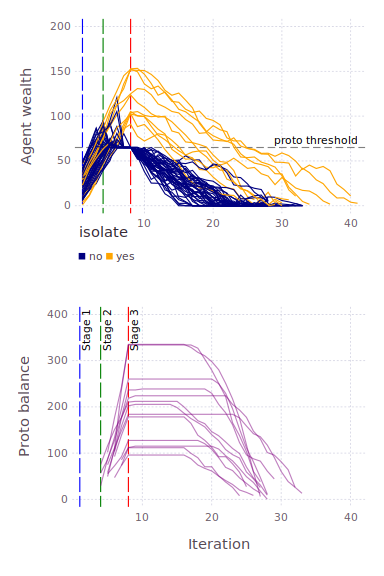
\includegraphics[width=\columnwidth]{figures/sampleLifeHistory.png}
\caption{A single run of the simulation, with $\lambda$=2. Each of 50 nodes is
given an initial wealth of $\sim\mathcal{U}(0,50)$ units, a regular income
distributed as $\sim\mathcal{N}(20,5)$, a metabolic rate of 5, and a proto
threshold of 65.} \label{fig:singleRun}
\end{figure}

This history can be seen in Figure~\ref{fig:singleRun}. The top plot depicts
agent wealth at every iteration, and the bottom plot shows the balances of the
protos at the same points in time. (No protos exist until stage 2, by
definition.) Note that the isolates (orange lines) never form protos, and
therefore begin the starvation stage with a higher personal wealth to draw
from.


\begin{figure}[ht]
\centering
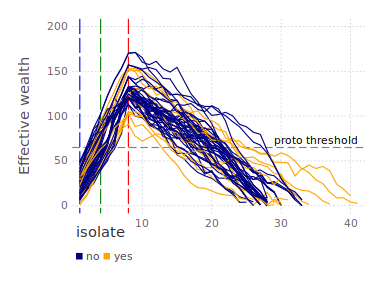
\includegraphics[width=\columnwidth]{figures/sampleEffectiveHistory.png}
\caption{The same simulation run as Figure~\ref{fig:singleRun}, but this time
depicting each agent's \textit{effective} wealth (its personal wealth plus its
share of its proto's wealth, if any).}
\label{fig:effectiveWealthSingleRun}
\end{figure}

Figure~\ref{fig:effectiveWealthSingleRun} shows the same information in another
way: instead of plotting each agent's \textit{personal} wealth (as in the top
plot of Figure~\ref{fig:singleRun}), we show its \textbf{effective wealth},
defined as the sum of its personal wealth and its ``share'' of its proto's
wealth (if any). After all, contributions that a proto's members make to its
balance are available to those members in times of need; therefore, a fair
comparison between isolates and non-isolates should take this into account.
From the figure, it can be seen that isolates no longer have a systematic
advantage (as they appeared to in Figure~\ref{fig:singleRun}.)

We verified that changes to basic parameters all have the expected effect:
lowering the initial wealth delays the onset of stage 2; a higher $\sigma^2$
for the income distribution makes the lines less jagged; a higher metabolic
rate hastens extinction; \textit{etc.}

\subsection{Gini coefficient history}

% Will's paragraph goes here, references Figure~\ref{fig:giniHistory}.

\begin{figure}[hb]
\centering
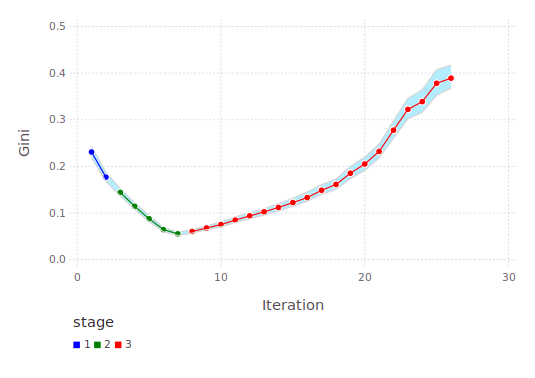
\includegraphics[width=\columnwidth]{figures/giniHistory.png}
\caption{The simulated society's wealth inequality over time. (The same
simulation parameters were used as in Figures~\ref{fig:singleRun} and
\ref{fig:effectiveWealthSingleRun}, but this time with 500 agents.) The light
blue band represents a bootstrapped 95\% confidence interval.}
\label{fig:giniHistory}
\end{figure}

    The Gini coefficient of the agent population as seen in the top plot of Figure~\ref{fig:giniHistory} is influenced by two distinct dynamics: loss/accumulation of wealth and the formation/death of proto-institutions. Over the course of Stage 1 and the beginning of Stage 3, this change in agent wealth is exclusively responsible for changes in the Gini coefficient. As agents accumulate wealth over Stage 1 and 2, the size of wealth differentials shrinks relative to absolute agent wealth, leading to the declining Gini coefficient. The opposite effect occurs during Stage 3 as agent starvation leads to the relative growth of these wealth differentials. The variability in starvation rates further stimulates the increasing Gini coefficient.

    In addition, as indicated in the bottom plot, the proto formation and proto death also influence the Gini coefficient during Stage 2 and the end of Stage 3, respectively. As expected, the formation of protos during Stage 2 contributes to declining Gini coefficient as the constituent agents of each proto have equivalent wealth values and represent coalitions of perfect economic equality. Accordingly, the death of protos, beginning around Iteration 20, contributes to increase the Gini coefficient by removing the protos' effect on the system's inequality. 

    (Note: As the population size decreases over the starvation period, the Gini coefficient becomes increasingly unstable and susceptible to small fluctuations in agent wealth; hence the erratic nature of the red line at the extreme right of Figure~\ref{fig:giniHistory}.)

% vim:textwidth=99999


\section{Analysis}
% (Separate analysis.tex file, so all images are in a separate file.)

First, we verify that the simulation's output matches obviously expected
results. Then, we investigate aspects of its behavior which are not computable
analytically in order to discover important consequences of the model.


\subsection{Verification}

\subsubsection{Single simulation runs}

For a sensible range of parameter settings, the life history of a single
simulation run follows an expected pattern. Assuming a positive growth rate
(\textit{i.e.}, salary > metabolic rate), each agent's wealth rises unsteadily
during stage 1, until eventually the first pair of neighboring agents who each
reach the threshold form a proto-institution. Throughout stage 2, these agents
contribute all wealth in excess of the threshold to that proto, and so their
proto's balance rises unsteadily while their personal wealth remains at the
constant threshold. Meanwhile, the other agents also reach the threshold at
various points in time, and also form or join protos, until every non-isolate
(that is, every node with at least one neighbor) is a member of a proto. Stage
3 (the starvation period) then commences, with isolates drawing on a greater
personal wealth than the non-isolates. When an isolate reaches zero wealth, it
dies; when a non-isolate reaches zero, it draws from its (shared) proto balance
until that too, reaches zero, and it dies.

\begin{figure}[ht]
\centering
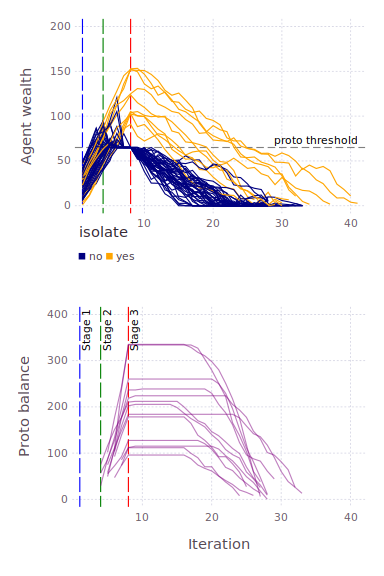
\includegraphics[width=\columnwidth]{figures/sampleLifeHistory.png}
\caption{A single run of the simulation, with $\lambda$=2. Each of 50 nodes is
given an initial wealth of 50 units, a regular income distributed as
$\sim\mathcal{N}(20,5)$, a metabolic rate of 5, and a proto threshold of 65.}
\label{fig:singleRun}
\end{figure}

This history can be seen in Figure~\ref{fig:singleRun}. The top plot depicts
agent wealth at every iteration, and the bottom plot shows the balances of the
protos at the same points in time. (No protos exist until stage 2, by
definition.) Note that the isolates (orange lines) never form protos, and
therefore begin the starvation stage with a higher personal wealth to draw
from.


\begin{figure}[ht]
\centering
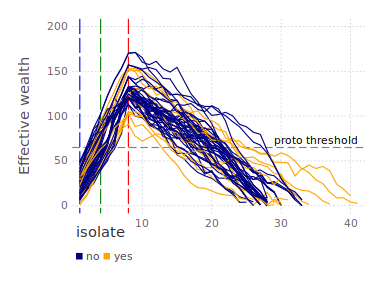
\includegraphics[width=\columnwidth]{figures/sampleEffectiveHistory.png}
\caption{The same simulation run as Figure~\ref{fig:singleRun}, but this time
depicting each agent's \textit{effective} wealth (its personal wealth plus its
share of its proto's wealth, if any).}
\label{fig:effectiveWealthSingleRun}
\end{figure}

Figure~\ref{fig:effectiveWealthSingleRun} shows the same information in another
way: instead of plotting each agent's \textit{personal} wealth (as in the top
plot of Figure~\ref{fig:singleRun}, we show its \textbf{effective wealth},
defined as the sum of its personal wealth and its ``share'' of its proto's
wealth (if any). After all, contributions that a proto's members make to its
balance are available to those members in times of need; therefore, a fair
comparison between isolates and non-isolates should take this into account.
From the figure, it can be seen that isolates no longer have a systematic
advantage (as they appeared to in Figure~\ref{fig:singleRun}.

We verified that changes to basic parameters all have the expected effect:
lowering the initial wealth delays the onset of stage 2; a higher $\sigma^2$
for the income distribution makes the lines less jagged; a higher metabolic
rate hastens extinction; \textit{etc.}


% Note that the empty graph can't really be shown because stages 2 and 3 have
% no well-defined meaning in that case.

% Show Gini plot, null hypothesis, "this is why it doesn't matter"

% Show different levels of white noise intensity relative to growth rate
%     (salary - metabolic rate)


\subsubsection{Parameter sweeps}

% Gini coefficient (pre-stage-3) decreases with λ

\subsection{Findings}

% Wealth histogram is steady ?

% Which is better strategy: to form protos when possible, or not?


\section{Conclusion and Future Work}
%%%%%%%%%%%%%%%%%%%%%%%%%%%%%%%%%%%%%%


%%%Idea for final section as of today 06/13 

%%%% Simulations cleary show systematic variations in both inequality and death time as both white noise and network parameter changes.... the precise interpretation and understanding of the phenomena at a more basic level is underwya.. more precise statistical tests are required... 

%%% Discuss how there are too many things to do along several fronts as this is at the interface of mathematics, simulation, economics and sociogy

% Discuss the importance of simple stylized models for use in computational economics ..... cite the papers of Testatsion, Wihtle and Arthur... tell how simple model provides insight into the economic systems... discuss the importance of not having equilibrium assumptions.....

%%% link to the use of these models to tease out actual social mechanisms as is warranted by analytical sociology 

%%%% Still, these models, at least the ones planned for the future are ideal for studying economic systems of small scale societies... cite the anthropology work....

%%% cite RV work where the idea of market forces start opearting only after a certain threshold.... and if everythin is below that threahold, there is no reason to expect that macroeconomic models are useful in any way shape or form 

%%%%  Economics of poverty is totally difference and is expected to involve completely different set of models... maybe use ideas from notes below 

%%%%%%%%%%%%%%%%%%%%%%%%%%%%%%%%%%%%%%%%%
%%%Things that could be discussed here but is redundant if we are running out of words 
%The general idea is to discuss how/why social networks matter wealth accumulation dynamics. We have references from anthropology. We have references in economic sociology(jackson).Sampson's work and Venkatesh's work can be used when talking about urban poverty and urban sociology. Discuss how in economics, wealth accumulation dynamics are mostly discussed at the macroeconomic level. In this sense, this work (and the work presented last year) are novel in this regard.  

%% Sampson's work seem to be crucial for making the claim that social structures and neighborhood effects are important determinants of economic outcomes. 

% Wealth accumulation models all start from fancy macroeconomic models and may not be well suited for studying wealth accumulation processes under poverty where high level of stochasticity seem to matter. 

%While we are interested in more sophisticated models, we are more interested in extracting the effects of social network structure in simple models of cooperative wealth accumulation. The proto-institution is definitely borrowed from SriMil. In order to study more elaborate and economically rigorous wealth dynamics, we need to be able sort of the effects of network structure in simple stylized network models. The work on ER models is expected to be first of our analysis. Eventually, we plan to get to more realistic wealth accumulation models of interest to economists but for now this is all we have.  

%In Katz's book, the differing life histories of individuals in Hamilton, Canada suggest that luck played a role in deterministic life outcomes. Katz argues that social mobility makes sense only in the context of social structure

%Katz's chapter 2. His main argument there is that the structure of inequality represent in Hamilton, Canada is representative of inequality present in all other north American cities of that era. The persistence of inequality can be see in the persistence of four kinds of social structures. 1) occupational structure, 2) division of wealth and proportion of the wealthy, 3) social and demographic identity of different economic ranks, and 4) distance between people of different socio-economic ranks or social stratification. He talks about persistence of networks of wealth and power. Points out strong interconnection between property, political power and social status. Argues that economic stratification and its crystallization leads to crystallization of social and other subjective stratifications.  



%%%%%%%%%%%%%%%%%%%%%%%%%%%%%%%%%%%%%%
%%%% This one is really important and top priority for use as a zoomed out conclusion 
%what kinds of real world systems are we talking about?This section should write itself. Just a brief discussion of phase 2+ and integration with spescape should suffice 
%%%% ERGM, SBM and LNM are good next steps 
%%%%% Use anthropology references to motivate more expressive models 
\cite{power2018cooperation,power2018}

\cite{koster2019,koster2014,koster2015,bogerhoff2015}

\cite{smith2019,nolin2012}


%%%% 

%%%%%%%%%%%%%%%%%%%%%%%%%%%%%%%%%
%I am actually confused about whether such a purely preliminary work can say antyhing about the real world. Do we really want to say anything at all about the real world. What can ER graphs say about the real world?  

%We conclude by discussing features of social processes and mechanisms argued for by both Sampson and Katz that are currently not present in the model but important and part of the vision for where our model is headed. 

%We also include the goal of seamlessly going from a model with no geography to a model with geography. 

% I am moving the discussion of connections to anthropology to this section 


\bibliography{ref_cssa19}
\end{document}
% this line is for Stephen's purposes only:
% vim:textwidth=99999
